\graphicspath{ {Figures/chapter05} }
\section{Introduction}
In this chapter, we'll show and confirm the outcomes of our modeling efforts, examining both the linear and non-linear states of the model. We'll compare these models with the real-world implementation and Simscape simulations. Next, we'll evaluate the performance of the PID controller we designed earlier in the previous chapter by comparing simulated results with our system actual outcomes.
\section{Open Loop Step Response of Linear and Non-linear Models against Real Implementation}
To ensure our model's accuracy, we conducted a step response comparison under Open Loop conditions, as depicted in Figure 5.1.
\begin{figure}[h]
    \centering
    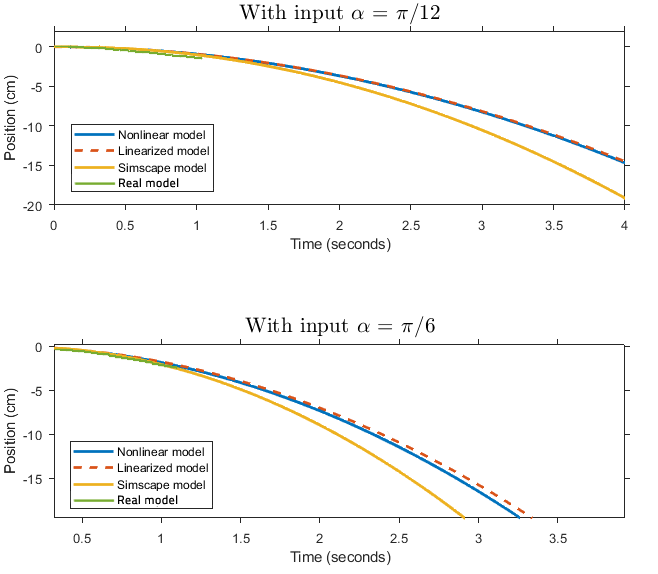
\includegraphics[width=1\linewidth]{Linearization_validation.png}
    \caption{open loop response comparison between the real plant, nonlinear model, linearized model, simscape model}
    \label{fig:enter-label}
\end{figure}
The Figure 5.1 indicate a clear instability in the system, particularly noticeable as the input angle rises. A noticeable difference arises between the linearized and non-linear systems. The observed difference can be traced back to our simplification assumption,  limiting the input plate inclination angle to the range of -15 to +15 degrees.Any variations beyond this specified range result in increased disparities between the linear and non-linear responses.

Moreover, our model assumes an infinite plate space, depicting a scenario where the ball neither falls nor bounces. This abstraction diverges from reality, introducing challenges and complexities in the practical implementation of the system

As a final test, the response of the real system to an angle of pi/12 is depicted in the figure 5.1. Notably, the response aligns reasonably well with our linear model, suggesting a certain level of reliability in our linearized representation

\section{Closed Loop Validation of PID Controller Performance}
In the tuning stage of our PID controller, achieving system stability was impossible  using only a P or PI controllers, The ball exhibited endless rolling or even falling off the plate.
therefore tuning a full PID controller was necessary, after  manual tuning process characterized by trial and error the parameter derived was  as shown in table 4.1. The resulting  experimental step responses of the three PIDs tuned parameters are depicted in Figure 5.2, and details of these responses characteristics are presented in Table 5.1, The experimental step responses in Figure 5.2 reveal distinct behaviors under the influence of PID1, PID2, and PID3. PID2, characterized by a 100\% overshoot and a relatively shorter rise time of 0.55 seconds, demonstrates a more aggressive response compared to PID1 and PID3.
\begin{table}[ht]
    \centering
    \caption{PID Controller Characteristics}
    \label{tab:pid-parameters}
    \begin{tabular}{|c|c|c|c|}
        \hline
        \textbf{Controller} & \textbf{Overshoot (\%)} & \textbf{Rise Time (s)} \\
        \hline
        PID1 & 20 & 0.65 \\
        PID2 & 100 & 0.55 \\
        PID3 & 28 & 0.65 \\
        \hline
    \end{tabular}
\end{table} 

the resulting simulation and experimental response and controller output for all three PIDs is in the figure 5.3, 5.4, and 5.5 a and b respectively, Between the two responses a and b of each figure there are subtle differences. This variance can be caused by factors such as the neglected friction, vibrations from the servomotor or plate, time delays caused by the filtering or data transmission, and the non-symmetry in the shape of the ball. These real-world complexities introduce nuances that impact the system's behavior.

\begin{figure}[h]
     \centering
     \begin{subfigure}[b]{0.95\textwidth}
         \centering
         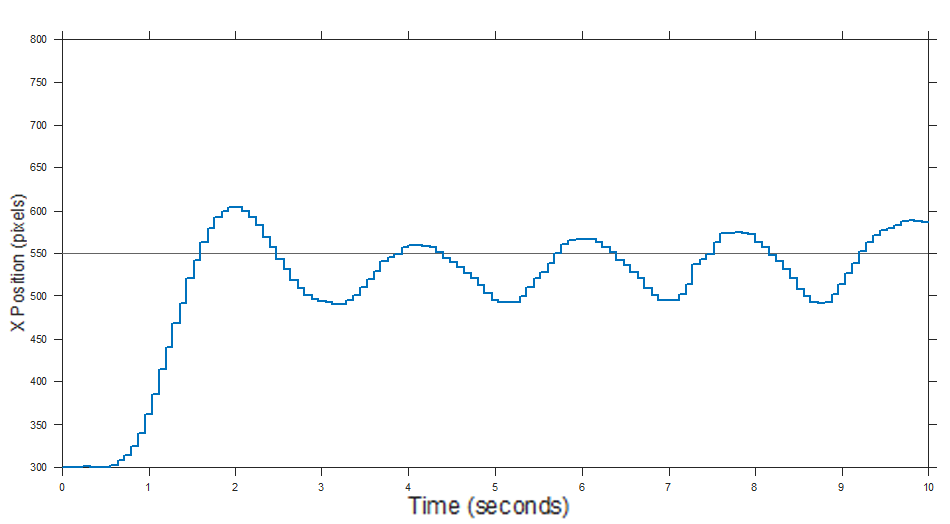
\includegraphics[width=\textwidth]{Step_response_PID1_Expiremental_x}
         \caption{PID Controller 1}
         \label{fig:y equals x}
     \end{subfigure}
     \hfill
     \begin{subfigure}[b]{0.95\textwidth}
         \centering
         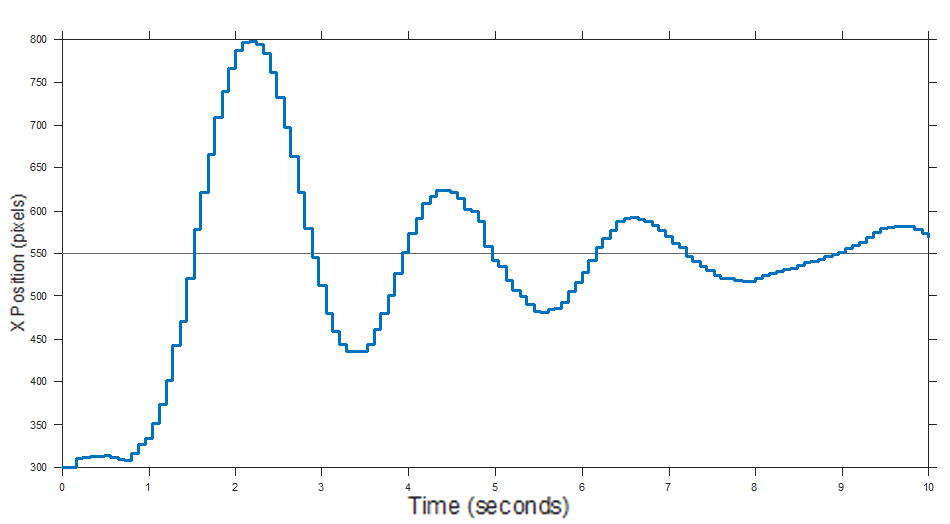
\includegraphics[width=\textwidth]{Step_response_PID2_Expiremental_x}
         \caption{PID Controller 2}
         \label{fig:three sin x}
     \end{subfigure}
     \hfill
     \begin{subfigure}[b]{0.95\textwidth}
         \centering
         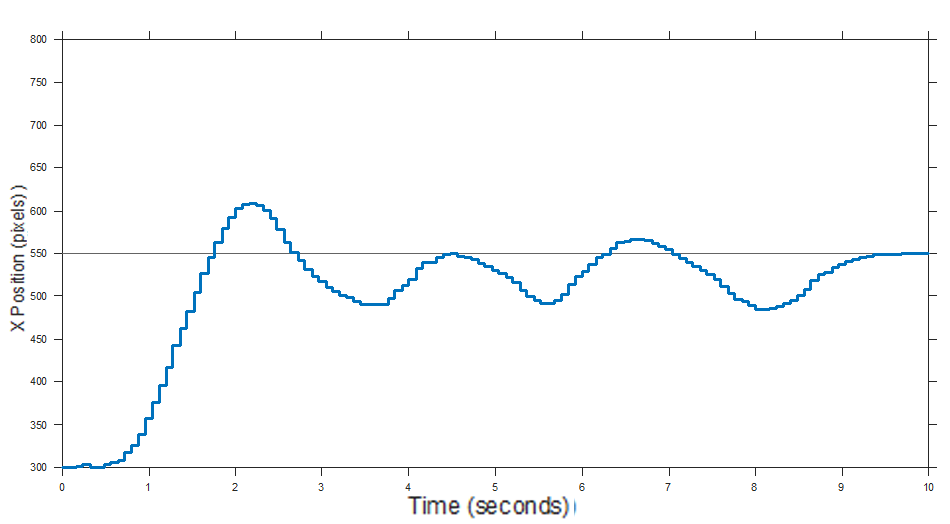
\includegraphics[width=\textwidth]{Step_response_PID3_Expiremental_x}
         \caption{PID Controller 3}
         \label{fig:five over x}
     \end{subfigure}
        \caption{Experimental Step Response and Control Output of the  BPS.}
        \label{fig:three graphs}
\end{figure}

\begin{figure}[h]
     \centering
     \begin{subfigure}[b]{1\textwidth}
         \centering
         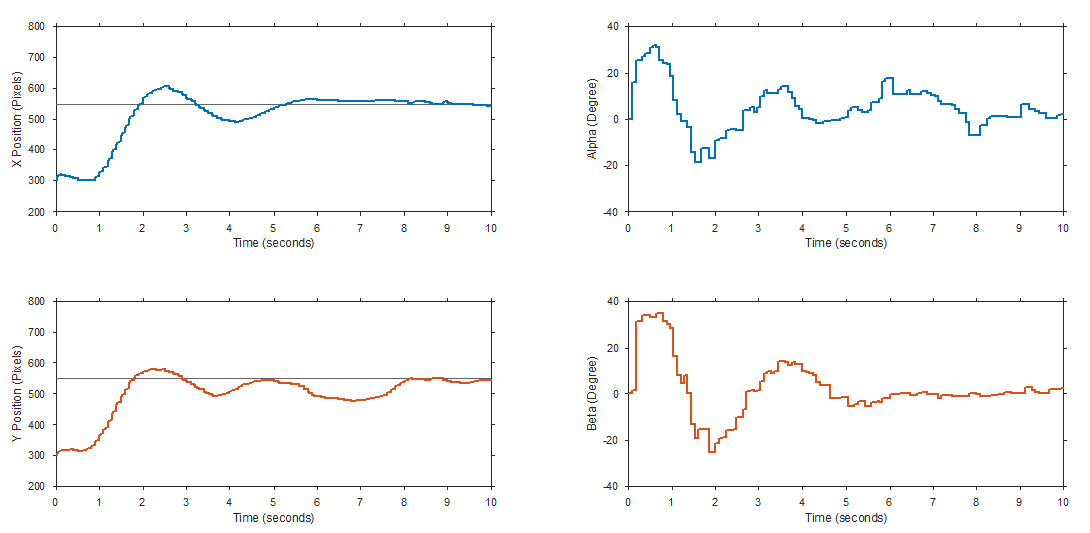
\includegraphics[width=\textwidth]{Figures/chapter05/Step_response_PID1_Expiremental.png}
         \caption{Experimental results}
         \label{fig:y equals x}
     \end{subfigure}
     \hfill
     \begin{subfigure}[b]{1\textwidth}
         \centering
         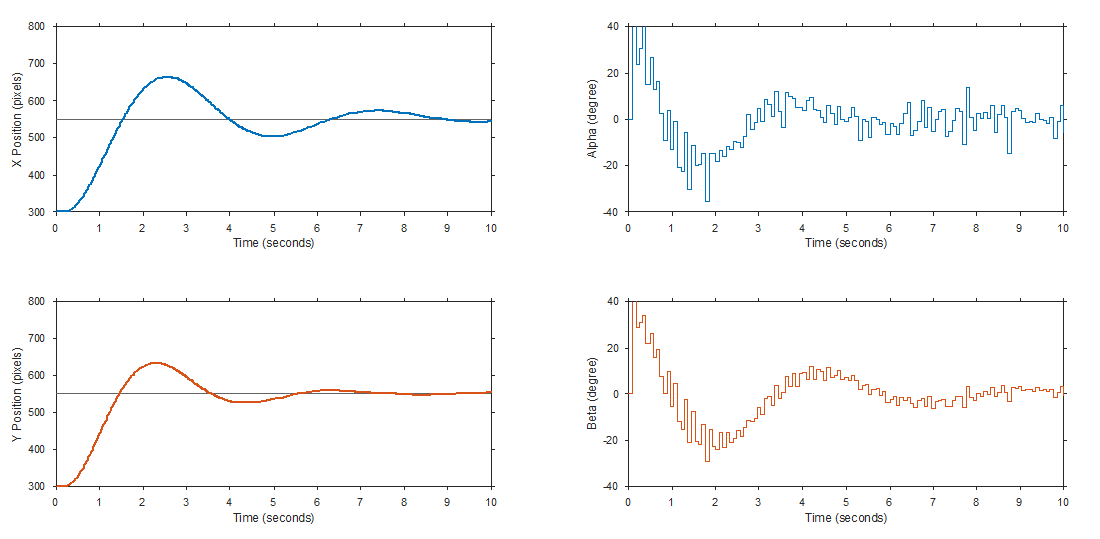
\includegraphics[width=\textwidth]{Figures/chapter05/Step_response_PID1_Simulation.png}
         \caption{Simulation result}
         \label{fig:three sin x}
     \end{subfigure}
        \caption{Step Response and Control Output of the  BPS under parameters of PID 1.}
        \label{fig:three graphs}
\end{figure}
\begin{figure}[h]
     \centering
     \begin{subfigure}[b]{1\textwidth}
         \centering
         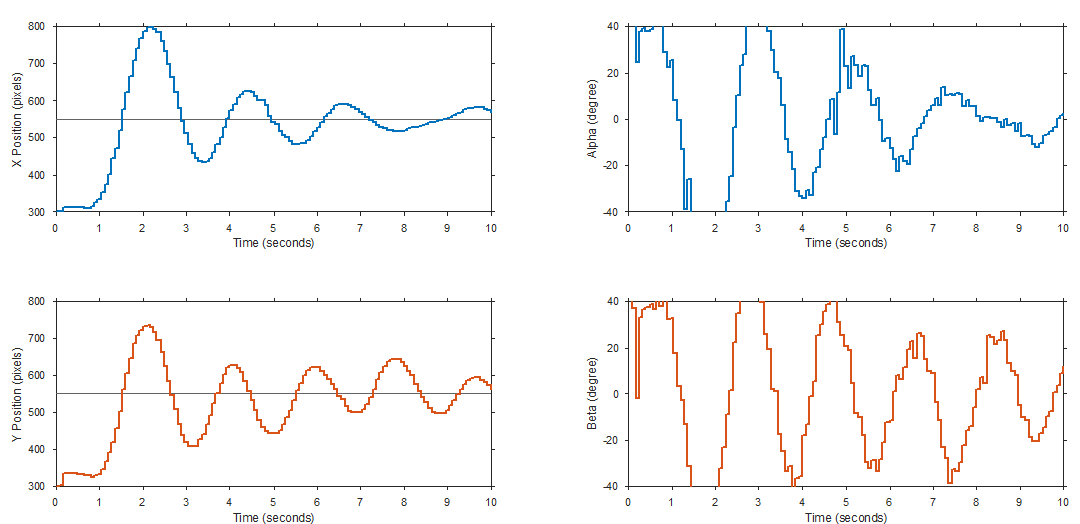
\includegraphics[width=\textwidth]{Figures/chapter05/Step_response_PID2_Expiremental.png}
         \caption{Experimental results}
         \label{fig:y equals x}
     \end{subfigure}
     \hfill
     \begin{subfigure}[b]{1\textwidth}
         \centering
         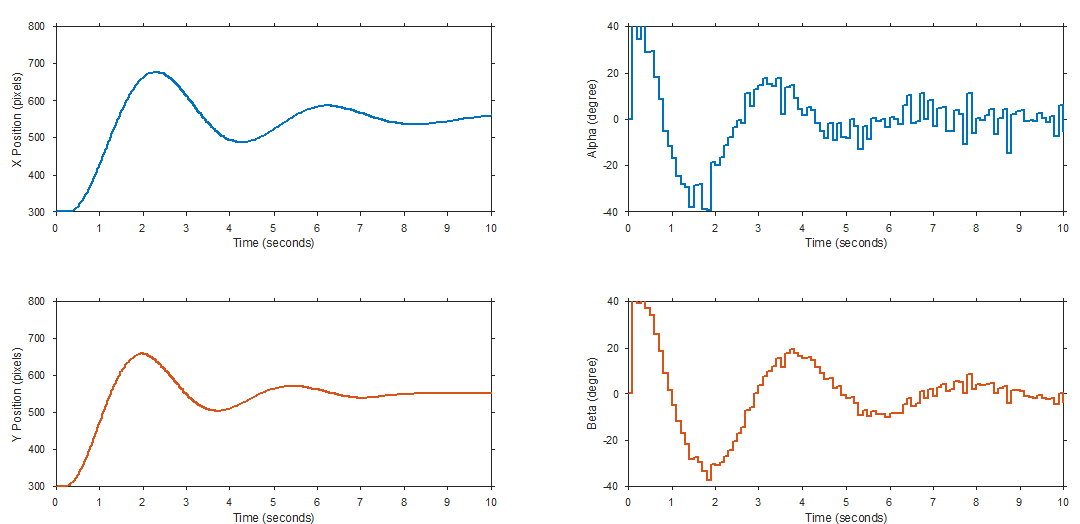
\includegraphics[width=\textwidth]{Figures/chapter05/Step_response_PID2_Simulation.png}
         \caption{Simulation result}
         \label{fig:three sin x}
     \end{subfigure}
        \caption{Step Response and Control Output of the BPS under parameters of PID 2.}
        \label{fig:three graphs}
\end{figure}
\begin{figure}[h]
     \centering
     \begin{subfigure}[b]{1\textwidth}
         \centering
         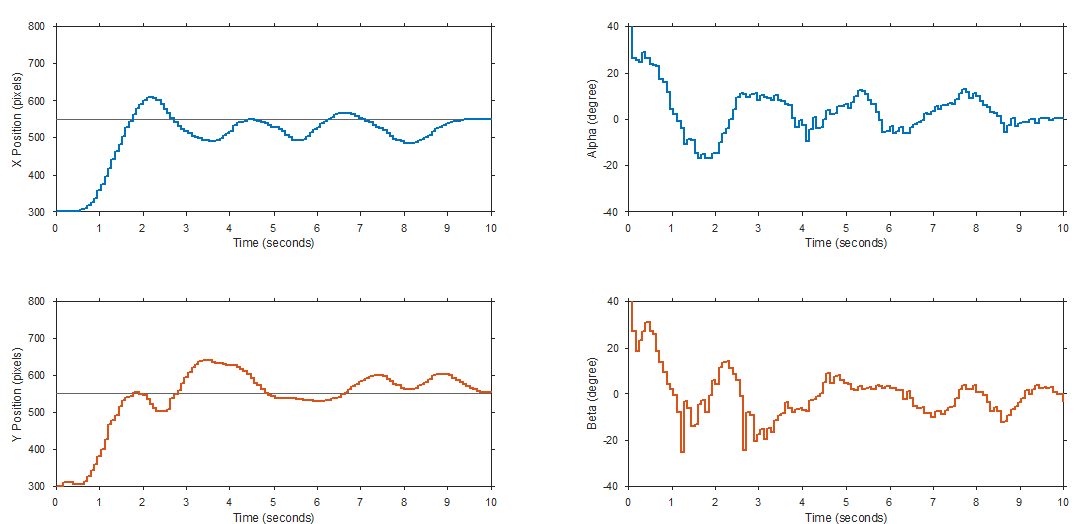
\includegraphics[width=\textwidth]{Figures/chapter05/Step_response_PID3_Expiremental.png}
         \caption{Experimental results}
         \label{fig:y equals x}
     \end{subfigure}
     \hfill
     \begin{subfigure}[b]{1\textwidth}
         \centering
         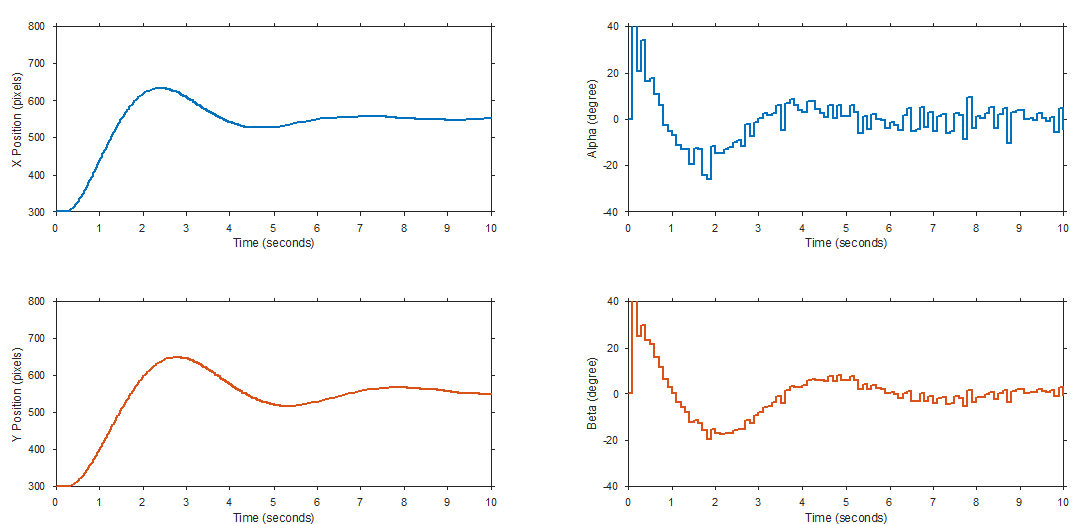
\includegraphics[width=\textwidth]{Figures/chapter05/Step_response_PID3_Simulation.png}
         \caption{Simulation result}
         \label{fig:three sin x}
     \end{subfigure}
        \caption{Step Response and Control Output of the  BPS under parameters of PID 3.}
        \label{fig:three graphs}
\end{figure}

The integral action in our controller can effectively eliminate steady-state errors, but the presence of steady-state error in the response caused by the static friction, When the ball gets close to the desired position, small tilting the plate might not be enough to overcome static friction. This can cause the ball to briefly get stuck, leading to a steady-state error that persists for a short time.
\begin{figure}[h]
     \centering
     \begin{subfigure}[b]{1\textwidth}
         \centering
         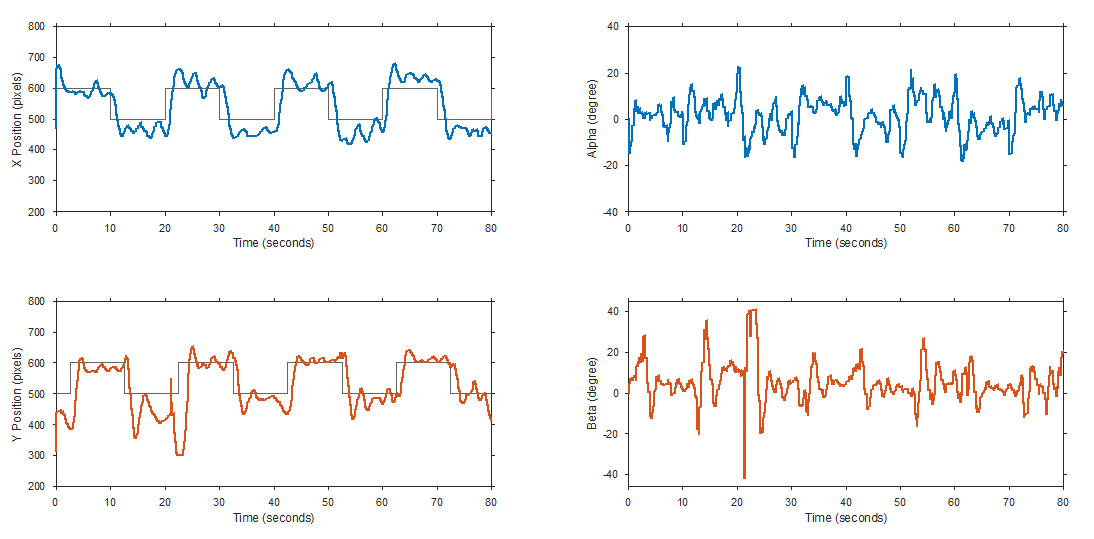
\includegraphics[width=\textwidth]{Figures/chapter05/square_tracking_PID1_Expiremental.png}
         \caption{Experimental results}
         \label{fig:y equals x}
     \end{subfigure}
     \hfill
     \begin{subfigure}[b]{1\textwidth}
         \centering
         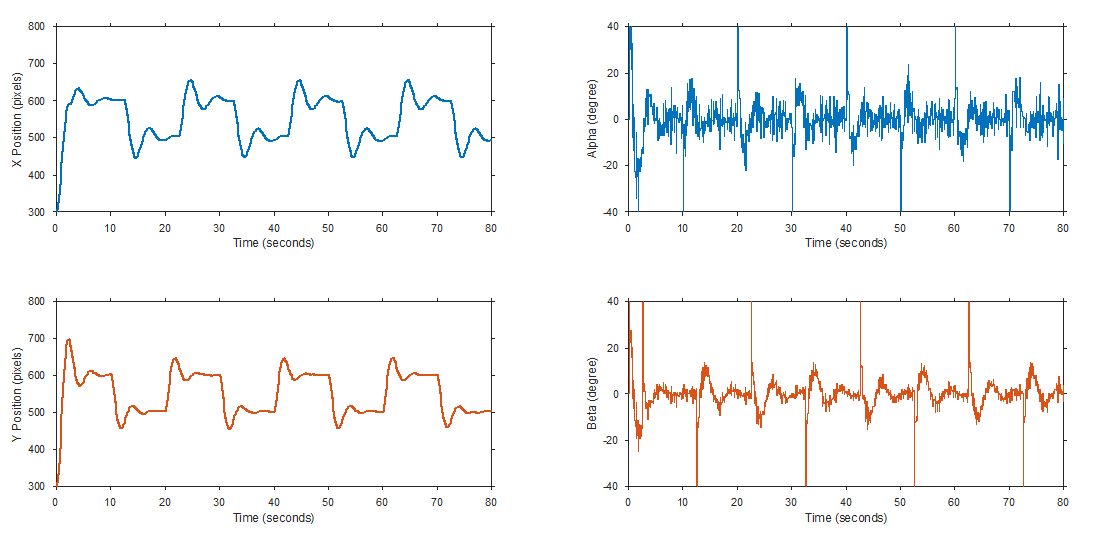
\includegraphics[width=\textwidth]{Figures/chapter05/square_tracking_PID1_simulation.png}
         \caption{Simulation result}
         \label{fig:three sin x}
     \end{subfigure}
        \caption{Square trajectory Response and Control Output of the  BPS under parameters of PID 1.}
        \label{fig:three graphs}
\end{figure}
\begin{figure}[h]
     \centering
     \begin{subfigure}[b]{1\textwidth}
         \centering
         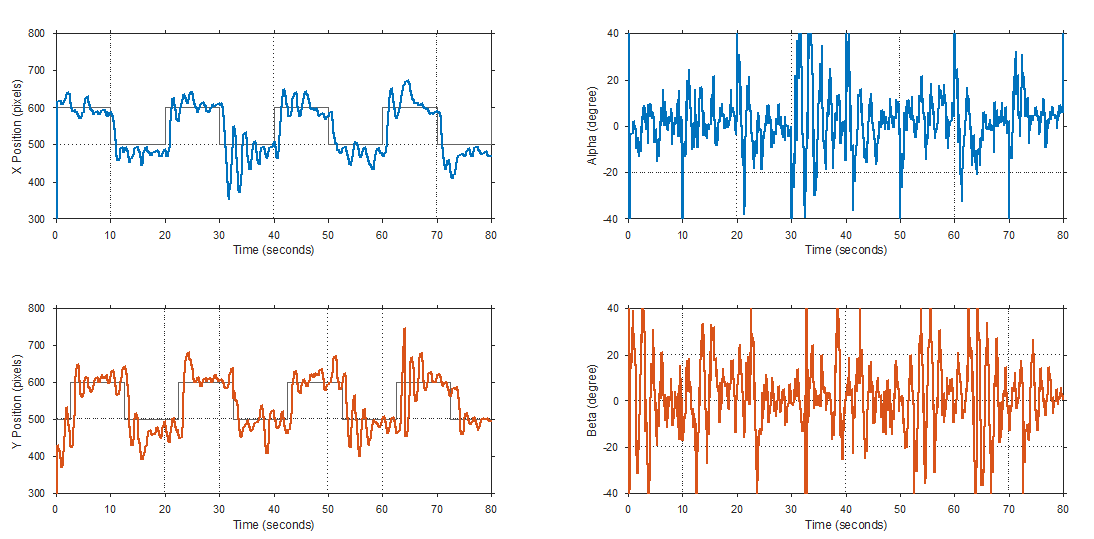
\includegraphics[width=\textwidth]{Figures/chapter05/square_tracking_PID2_Expiremental.png}
         \caption{Experimental results}
         \label{fig:y equals x}
     \end{subfigure}
     \hfill
     \begin{subfigure}[b]{1\textwidth}
         \centering
         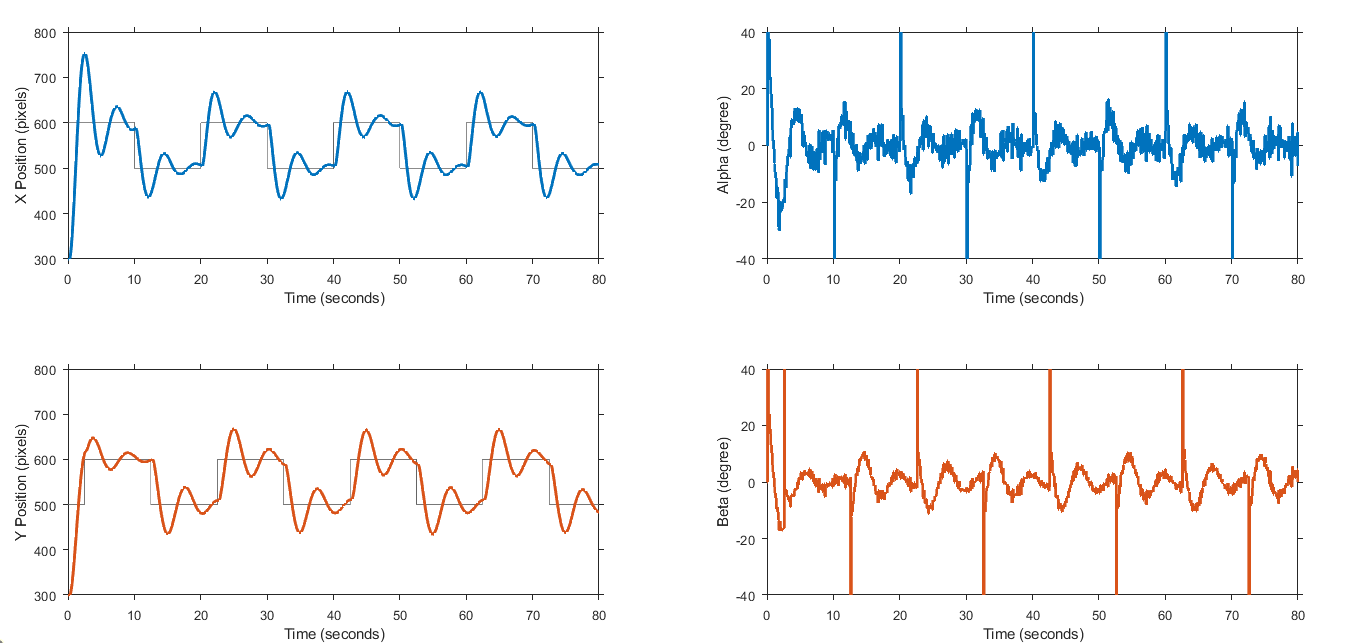
\includegraphics[width=\textwidth]{Figures/chapter05/square_tracking_PID2_simulation.png}
         \caption{Simulation result}
         \label{fig:three sin x}
     \end{subfigure}
        \caption{Square trajectory Response and Control Output of the  BPS under parameters of PID 2.}
        \label{fig:three graphs}
\end{figure}
\begin{figure}[h]
     \centering
     \begin{subfigure}[b]{1\textwidth}
         \centering
         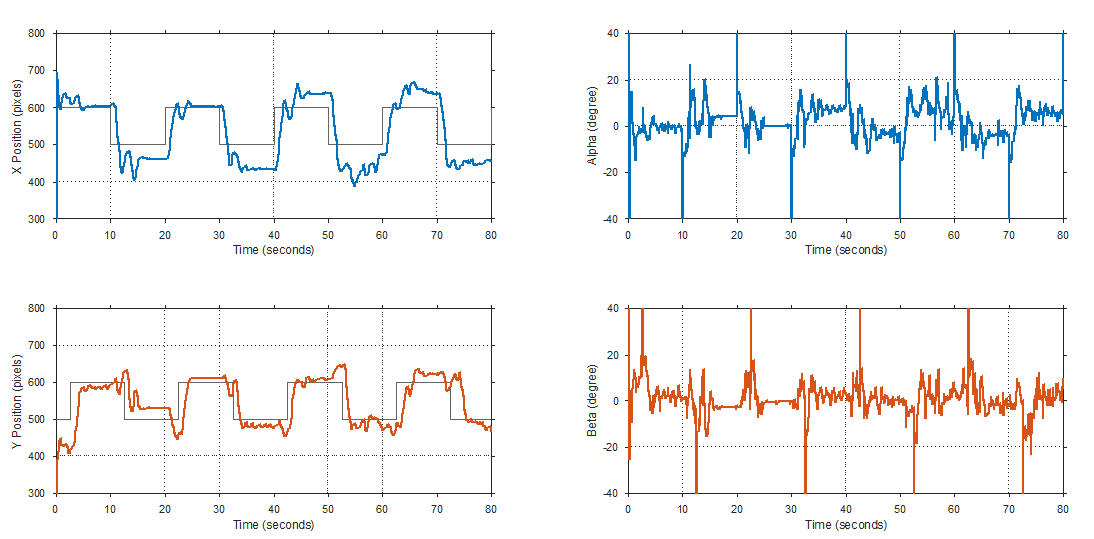
\includegraphics[width=\textwidth]{Figures/chapter05/square_tracking_PID3_Expiremental.png}
         \caption{Experimental results}
         \label{fig:y equals x}
     \end{subfigure}
     \hfill
     \begin{subfigure}[b]{1\textwidth}
         \centering
         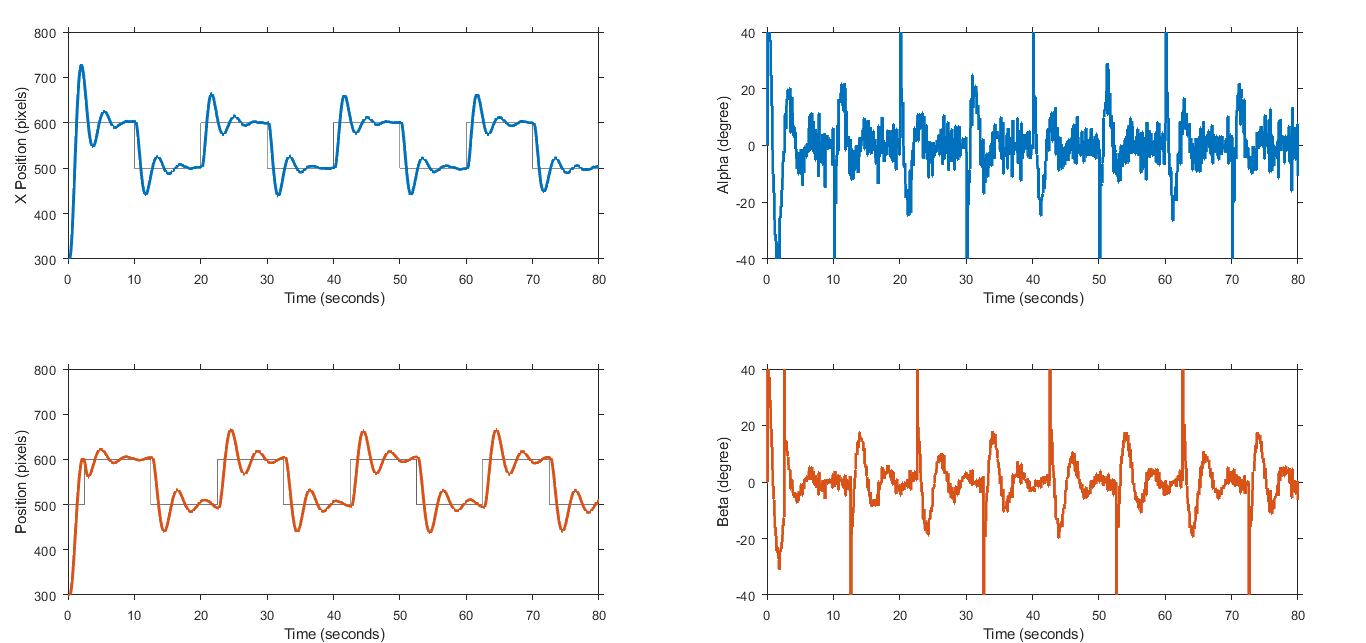
\includegraphics[width=\textwidth]{Figures/chapter05/square_tracking_PID3_simulation.png}
         \caption{Simulation result}
         \label{fig:three sin x}
     \end{subfigure}
        \caption{Square trajectory Response and Control Output of the  BPS under parameters of PID 3.}
        \label{fig:three graphs}
\end{figure}
The step response is always good to clearly see the quality of the controller’s performance, however, the plant should be able to track any reference given to it. The tracking of a square wave reference is shown in fig 5.6, 5.7, 5.8 a and b.
The issue of derivative kick is cearly shown in the control output of the figures when the angle of the controller goes extreme due to a sudden change in the input and it represent a major defect in PIDs controllers




